\documentclass[]{article}
\usepackage{lmodern}
\usepackage{amssymb,amsmath}
\usepackage{ifxetex,ifluatex}
\usepackage{fixltx2e} % provides \textsubscript
\ifnum 0\ifxetex 1\fi\ifluatex 1\fi=0 % if pdftex
  \usepackage[T1]{fontenc}
  \usepackage[utf8]{inputenc}
\else % if luatex or xelatex
  \ifxetex
    \usepackage{mathspec}
  \else
    \usepackage{fontspec}
  \fi
  \defaultfontfeatures{Ligatures=TeX,Scale=MatchLowercase}
\fi
% use upquote if available, for straight quotes in verbatim environments
\IfFileExists{upquote.sty}{\usepackage{upquote}}{}
% use microtype if available
\IfFileExists{microtype.sty}{%
\usepackage{microtype}
\UseMicrotypeSet[protrusion]{basicmath} % disable protrusion for tt fonts
}{}
\usepackage[margin=1in]{geometry}
\usepackage{hyperref}
\hypersetup{unicode=true,
            pdftitle={Supplementary figures and tables},
            pdfauthor={Popa-Baez A. D., Lee S. F., Yeap H. L., Prasad S. S., Schiffer M., Mourant R., Castro-Vargas C., Edwards O. R., Taylor P. W. and Oakeshott J. G.},
            pdfborder={0 0 0},
            breaklinks=true}
\urlstyle{same}  % don't use monospace font for urls
\usepackage{longtable,booktabs}
\usepackage{graphicx,grffile}
\makeatletter
\def\maxwidth{\ifdim\Gin@nat@width>\linewidth\linewidth\else\Gin@nat@width\fi}
\def\maxheight{\ifdim\Gin@nat@height>\textheight\textheight\else\Gin@nat@height\fi}
\makeatother
% Scale images if necessary, so that they will not overflow the page
% margins by default, and it is still possible to overwrite the defaults
% using explicit options in \includegraphics[width, height, ...]{}
\setkeys{Gin}{width=\maxwidth,height=\maxheight,keepaspectratio}
\IfFileExists{parskip.sty}{%
\usepackage{parskip}
}{% else
\setlength{\parindent}{0pt}
\setlength{\parskip}{6pt plus 2pt minus 1pt}
}
\setlength{\emergencystretch}{3em}  % prevent overfull lines
\providecommand{\tightlist}{%
  \setlength{\itemsep}{0pt}\setlength{\parskip}{0pt}}
\setcounter{secnumdepth}{0}
% Redefines (sub)paragraphs to behave more like sections
\ifx\paragraph\undefined\else
\let\oldparagraph\paragraph
\renewcommand{\paragraph}[1]{\oldparagraph{#1}\mbox{}}
\fi
\ifx\subparagraph\undefined\else
\let\oldsubparagraph\subparagraph
\renewcommand{\subparagraph}[1]{\oldsubparagraph{#1}\mbox{}}
\fi

%%% Use protect on footnotes to avoid problems with footnotes in titles
\let\rmarkdownfootnote\footnote%
\def\footnote{\protect\rmarkdownfootnote}

%%% Change title format to be more compact
\usepackage{titling}

% Create subtitle command for use in maketitle
\providecommand{\subtitle}[1]{
  \posttitle{
    \begin{center}\large#1\end{center}
    }
}

\setlength{\droptitle}{-2em}

  \title{Supplementary figures and tables}
    \pretitle{\vspace{\droptitle}\centering\huge}
  \posttitle{\par}
  \subtitle{Variation in stress tolerance in the Queensland fruit fly}
  \author{Popa-Baez A. D., Lee S. F., Yeap H. L., Prasad S. S., Schiffer M.,
Mourant R., Castro-Vargas C., Edwards O. R., Taylor P. W. and Oakeshott
J. G.}
    \preauthor{\centering\large\emph}
  \postauthor{\par}
      \predate{\centering\large\emph}
  \postdate{\par}
    \date{20 April 2019}

\usepackage{lscape}
\newcommand{\blandscape}{\begin{landscape}}
\newcommand{\elandscape}{\end{landscape}}
\renewcommand{\figurename}{\textbf{Figure S}}
\renewcommand{\tablename}{\textbf{Table S}}
\usepackage{booktabs}
\usepackage{longtable}
\usepackage{array}
\usepackage{multirow}
\usepackage{wrapfig}
\usepackage{float}
\usepackage{colortbl}
\usepackage{pdflscape}
\usepackage{tabu}
\usepackage{threeparttable}
\usepackage{threeparttablex}
\usepackage[normalem]{ulem}
\usepackage{makecell}
\usepackage{xcolor}

\begin{document}
\maketitle

\begin{longtable}[]{@{}llll@{}}
\caption{\textbf{Helper functions and packages in R used in the statistical analyses}}\tabularnewline
\toprule
~ & \textbf{R session information:} & ~ & ~\tabularnewline
\midrule
\endfirsthead
\toprule
~ & \textbf{R session information:} & ~ & ~\tabularnewline
\midrule
\endhead
\textbf{Based Packages attached:} & & &\tabularnewline
& grid & stats & graphics\tabularnewline
& methods & base & grDevices utils\tabularnewline
& datasets & &\tabularnewline
\textbf{Attached Packages:} & & &\tabularnewline
& wesanderson\_0.3.6 & readr\_1.3.1 & boot\_1.3-20\tabularnewline
& nortest\_1.0-4 & jtrans\_0.2.1 & Hmisc\_4.2-0\tabularnewline
& Formula\_1.2-3 & survival\_2.43-3 & lattice\_0.20-35\tabularnewline
& xtable\_1.8-3 & psych\_1.8.12 & egg\_0.4.2\tabularnewline
& gridExtra\_2.3 & sp\_1.3-1 & ggalluvial\_0.9.1\tabularnewline
& purrr\_0.3.0 & stargazer\_5.2.2 & cowplot\_0.9.4\tabularnewline
& magrittr\_1.5 & ggridges\_0.5.1 & ggplot2\_3.1.0\tabularnewline
& dplyr\_0.8.0 & emmeans\_1.3.3.0999901 &
RColorBrewer\_1.1-2\tabularnewline
& ggpubr\_0.2 & &\tabularnewline
\textbf{Packages loaded via namespace} & & &\tabularnewline
& httr\_1.4.0 & tidyr\_0.8.2 & viridisLite\_0.3.0\tabularnewline
& splines\_3.4.4 & assertthat\_0.2.0 & highr\_0.7\tabularnewline
& latticeExtra\_0.6-28 & yaml\_2.2.0 & sessioninfo\_1.1.1\tabularnewline
& pillar\_1.3.1 & backports\_1.1.3 & glue\_1.3.0\tabularnewline
& digest\_0.6.18 & checkmate\_1.9.1 & rvest\_0.3.2\tabularnewline
& colorspace\_1.4-0 & sandwich\_2.5-0 & captioner\_2.2.3\tabularnewline
& htmltools\_0.3.6 & Matrix\_1.2-14 & plyr\_1.8.4\tabularnewline
& pkgconfig\_2.0.2 & mvtnorm\_1.0-8 & webshot\_0.5.1\tabularnewline
& scales\_1.0.0 & htmlTable\_1.13.1 & tibble\_2.0.1\tabularnewline
& TH.data\_1.0-10 & withr\_2.1.2 & nnet\_7.3-12\tabularnewline
& lazyeval\_0.2.1 & cli\_1.0.1 & mnormt\_1.5-5\tabularnewline
& crayon\_1.3.4 & estimability\_1.3 & evaluate\_0.13\tabularnewline
& fansi\_0.4.0 & nlme\_3.1-137 & MASS\_7.3-50\tabularnewline
& xml2\_1.2.0 & foreign\_0.8-70 & tools\_3.4.4\tabularnewline
& data.table\_1.12.0 & hms\_0.4.2 & multcomp\_1.4-8\tabularnewline
& stringr\_1.4.0 & munsell\_0.5.0 & cluster\_2.0.7-1\tabularnewline
& kableExtra\_1.0.1 & compiler\_3.4.4 & rlang\_0.3.1\tabularnewline
& rstudioapi\_0.9.0 & htmlwidgets\_1.3 & labeling\_0.3\tabularnewline
& base64enc\_0.1-3 & rmarkdown\_1.11 & gtable\_0.2.0\tabularnewline
& codetools\_0.2-15 & R6\_2.3.0 & zoo\_1.8-4\tabularnewline
& knitr\_1.21 & utf8\_1.1.4 & stringi\_1.3.1\tabularnewline
& parallel\_3.4.4 & Rcpp\_1.0.0 & rpart\_4.1-13\tabularnewline
& acepack\_1.4.1 & tidyselect\_0.2.5 & xfun\_0.4\tabularnewline
& coda\_0.19-2 & &\tabularnewline
\bottomrule
\end{longtable}

\newpage

\begin{longtable}[]{@{}lll@{}}
\caption{\textbf{Methodological differences between the standard desiccation tolerance assay and that used for the resampled 2017/2018 collection}}\tabularnewline
\toprule
\begin{minipage}[b]{0.24\columnwidth}\raggedright\strut
Difference in protocol\strut
\end{minipage} & \begin{minipage}[b]{0.33\columnwidth}\raggedright\strut
First collection\strut
\end{minipage} & \begin{minipage}[b]{0.34\columnwidth}\raggedright\strut
Resampled collection\strut
\end{minipage}\tabularnewline
\midrule
\endfirsthead
\toprule
\begin{minipage}[b]{0.24\columnwidth}\raggedright\strut
Difference in protocol\strut
\end{minipage} & \begin{minipage}[b]{0.33\columnwidth}\raggedright\strut
First collection\strut
\end{minipage} & \begin{minipage}[b]{0.34\columnwidth}\raggedright\strut
Resampled collection\strut
\end{minipage}\tabularnewline
\midrule
\endhead
\begin{minipage}[t]{0.24\columnwidth}\raggedright\strut
Egg collection\strut
\end{minipage} & \begin{minipage}[t]{0.33\columnwidth}\raggedright\strut
Egging device\strut
\end{minipage} & \begin{minipage}[t]{0.34\columnwidth}\raggedright\strut
Baby (vine) capsicum\strut
\end{minipage}\tabularnewline
\begin{minipage}[t]{0.24\columnwidth}\raggedright\strut
Larvae rearing\strut
\end{minipage} & \begin{minipage}[t]{0.33\columnwidth}\raggedright\strut
Gel diet (Mohadeli et al., 2017)\strut
\end{minipage} & \begin{minipage}[t]{0.34\columnwidth}\raggedright\strut
Gel diet and baby (vine) capsicum\strut
\end{minipage}\tabularnewline
\begin{minipage}[t]{0.24\columnwidth}\raggedright\strut
Tubes\strut
\end{minipage} & \begin{minipage}[t]{0.33\columnwidth}\raggedright\strut
5 mL\strut
\end{minipage} & \begin{minipage}[t]{0.34\columnwidth}\raggedright\strut
10 mL\strut
\end{minipage}\tabularnewline
\begin{minipage}[t]{0.24\columnwidth}\raggedright\strut
Desiccant\strut
\end{minipage} & \begin{minipage}[t]{0.33\columnwidth}\raggedright\strut
8 silica gel beads\strut
\end{minipage} & \begin{minipage}[t]{0.34\columnwidth}\raggedright\strut
0.5g silica gel packet\strut
\end{minipage}\tabularnewline
\begin{minipage}[t]{0.24\columnwidth}\raggedright\strut
Scoring after 16 hours\strut
\end{minipage} & \begin{minipage}[t]{0.33\columnwidth}\raggedright\strut
Every 2 hours\strut
\end{minipage} & \begin{minipage}[t]{0.34\columnwidth}\raggedright\strut
Every 3 hours\strut
\end{minipage}\tabularnewline
\bottomrule
\end{longtable}

\newpage

\begin{table}[t]

\caption{\label{tab:S3 Table}\textbf{Individal populations for which the wild (G2/G3) and domesticated (G10-15) bioassay results differed signficantly.} Contrast are calculated for the estimated mean response variable for each population by looking at the differences of the domesticated over the wild populations. The estimated mean of teh contrast are calculated on the log transformed data for the response variables}
\centering
\begin{tabular}{lrrrr}
\toprule
Population & ratio & SE & z.ratio & p.value\\
\midrule
\addlinespace[0.3em]
\multicolumn{5}{l}{\textbf{Heat}}\\
\hspace{1em}Alice Springs & 1.09 & 0.09 & 1.07 & 0.28\\
\hspace{1em}Batemans Bay & 1.17 & 0.09 & 2.01 & 0.04\\
\hspace{1em}Brisbane & 1.17 & 0.09 & 1.97 & 0.05\\
\hspace{1em}Darwin & 1.10 & 0.09 & 1.19 & 0.23\\
\hspace{1em}Griffith & 1.21 & 0.10 & 2.42 & 0.02\\
\hspace{1em}Mareeba & 1.20 & 0.10 & 2.22 & 0.03\\
\hspace{1em}Narrabri & 1.10 & 0.09 & 1.20 & 0.23\\
\hspace{1em}Sydney & 1.09 & 0.08 & 1.05 & 0.29\\
\hspace{1em}Utchee Creek & 1.14 & 0.09 & 1.66 & 0.10\\
\addlinespace[0.3em]
\multicolumn{5}{l}{\textbf{Desiccation}}\\
\hspace{1em}Alice Springs & 0.68 & 0.05 & -5.74 & 0.00\\
\hspace{1em}Batemans Bay & 1.02 & 0.07 & 0.27 & 0.79\\
\hspace{1em}Brisbane & 1.07 & 0.07 & 1.05 & 0.29\\
\hspace{1em}Griffith & 0.90 & 0.06 & -1.56 & 0.12\\
\hspace{1em}Mareeba & 0.94 & 0.06 & -0.93 & 0.35\\
\hspace{1em}Narrabri & 1.23 & 0.08 & 3.04 & 0.00\\
\hspace{1em}Sydney & 0.54 & 0.04 & -9.37 & 0.00\\
\hspace{1em}Utchee Creek & 1.04 & 0.07 & 0.59 & 0.55\\
\addlinespace[0.3em]
\multicolumn{5}{l}{\textbf{Starvation}}\\
\hspace{1em}Alice Springs & 0.79 & 0.07 & -2.70 & 0.01\\
\hspace{1em}Batemans Bay & 0.92 & 0.09 & -0.86 & 0.39\\
\hspace{1em}Brisbane & 0.94 & 0.09 & -0.71 & 0.48\\
\hspace{1em}Griffith & 0.83 & 0.08 & -2.10 & 0.04\\
\hspace{1em}Mareeba & 0.95 & 0.09 & -0.59 & 0.56\\
\hspace{1em}Narrabri & 0.91 & 0.08 & -1.05 & 0.29\\
\hspace{1em}Sydney & 0.57 & 0.05 & -6.37 & 0.00\\
\hspace{1em}Utchee Creek & 0.89 & 0.08 & -1.31 & 0.19\\
\bottomrule
\end{tabular}
\end{table}

\newpage

\begin{figure}

{\centering 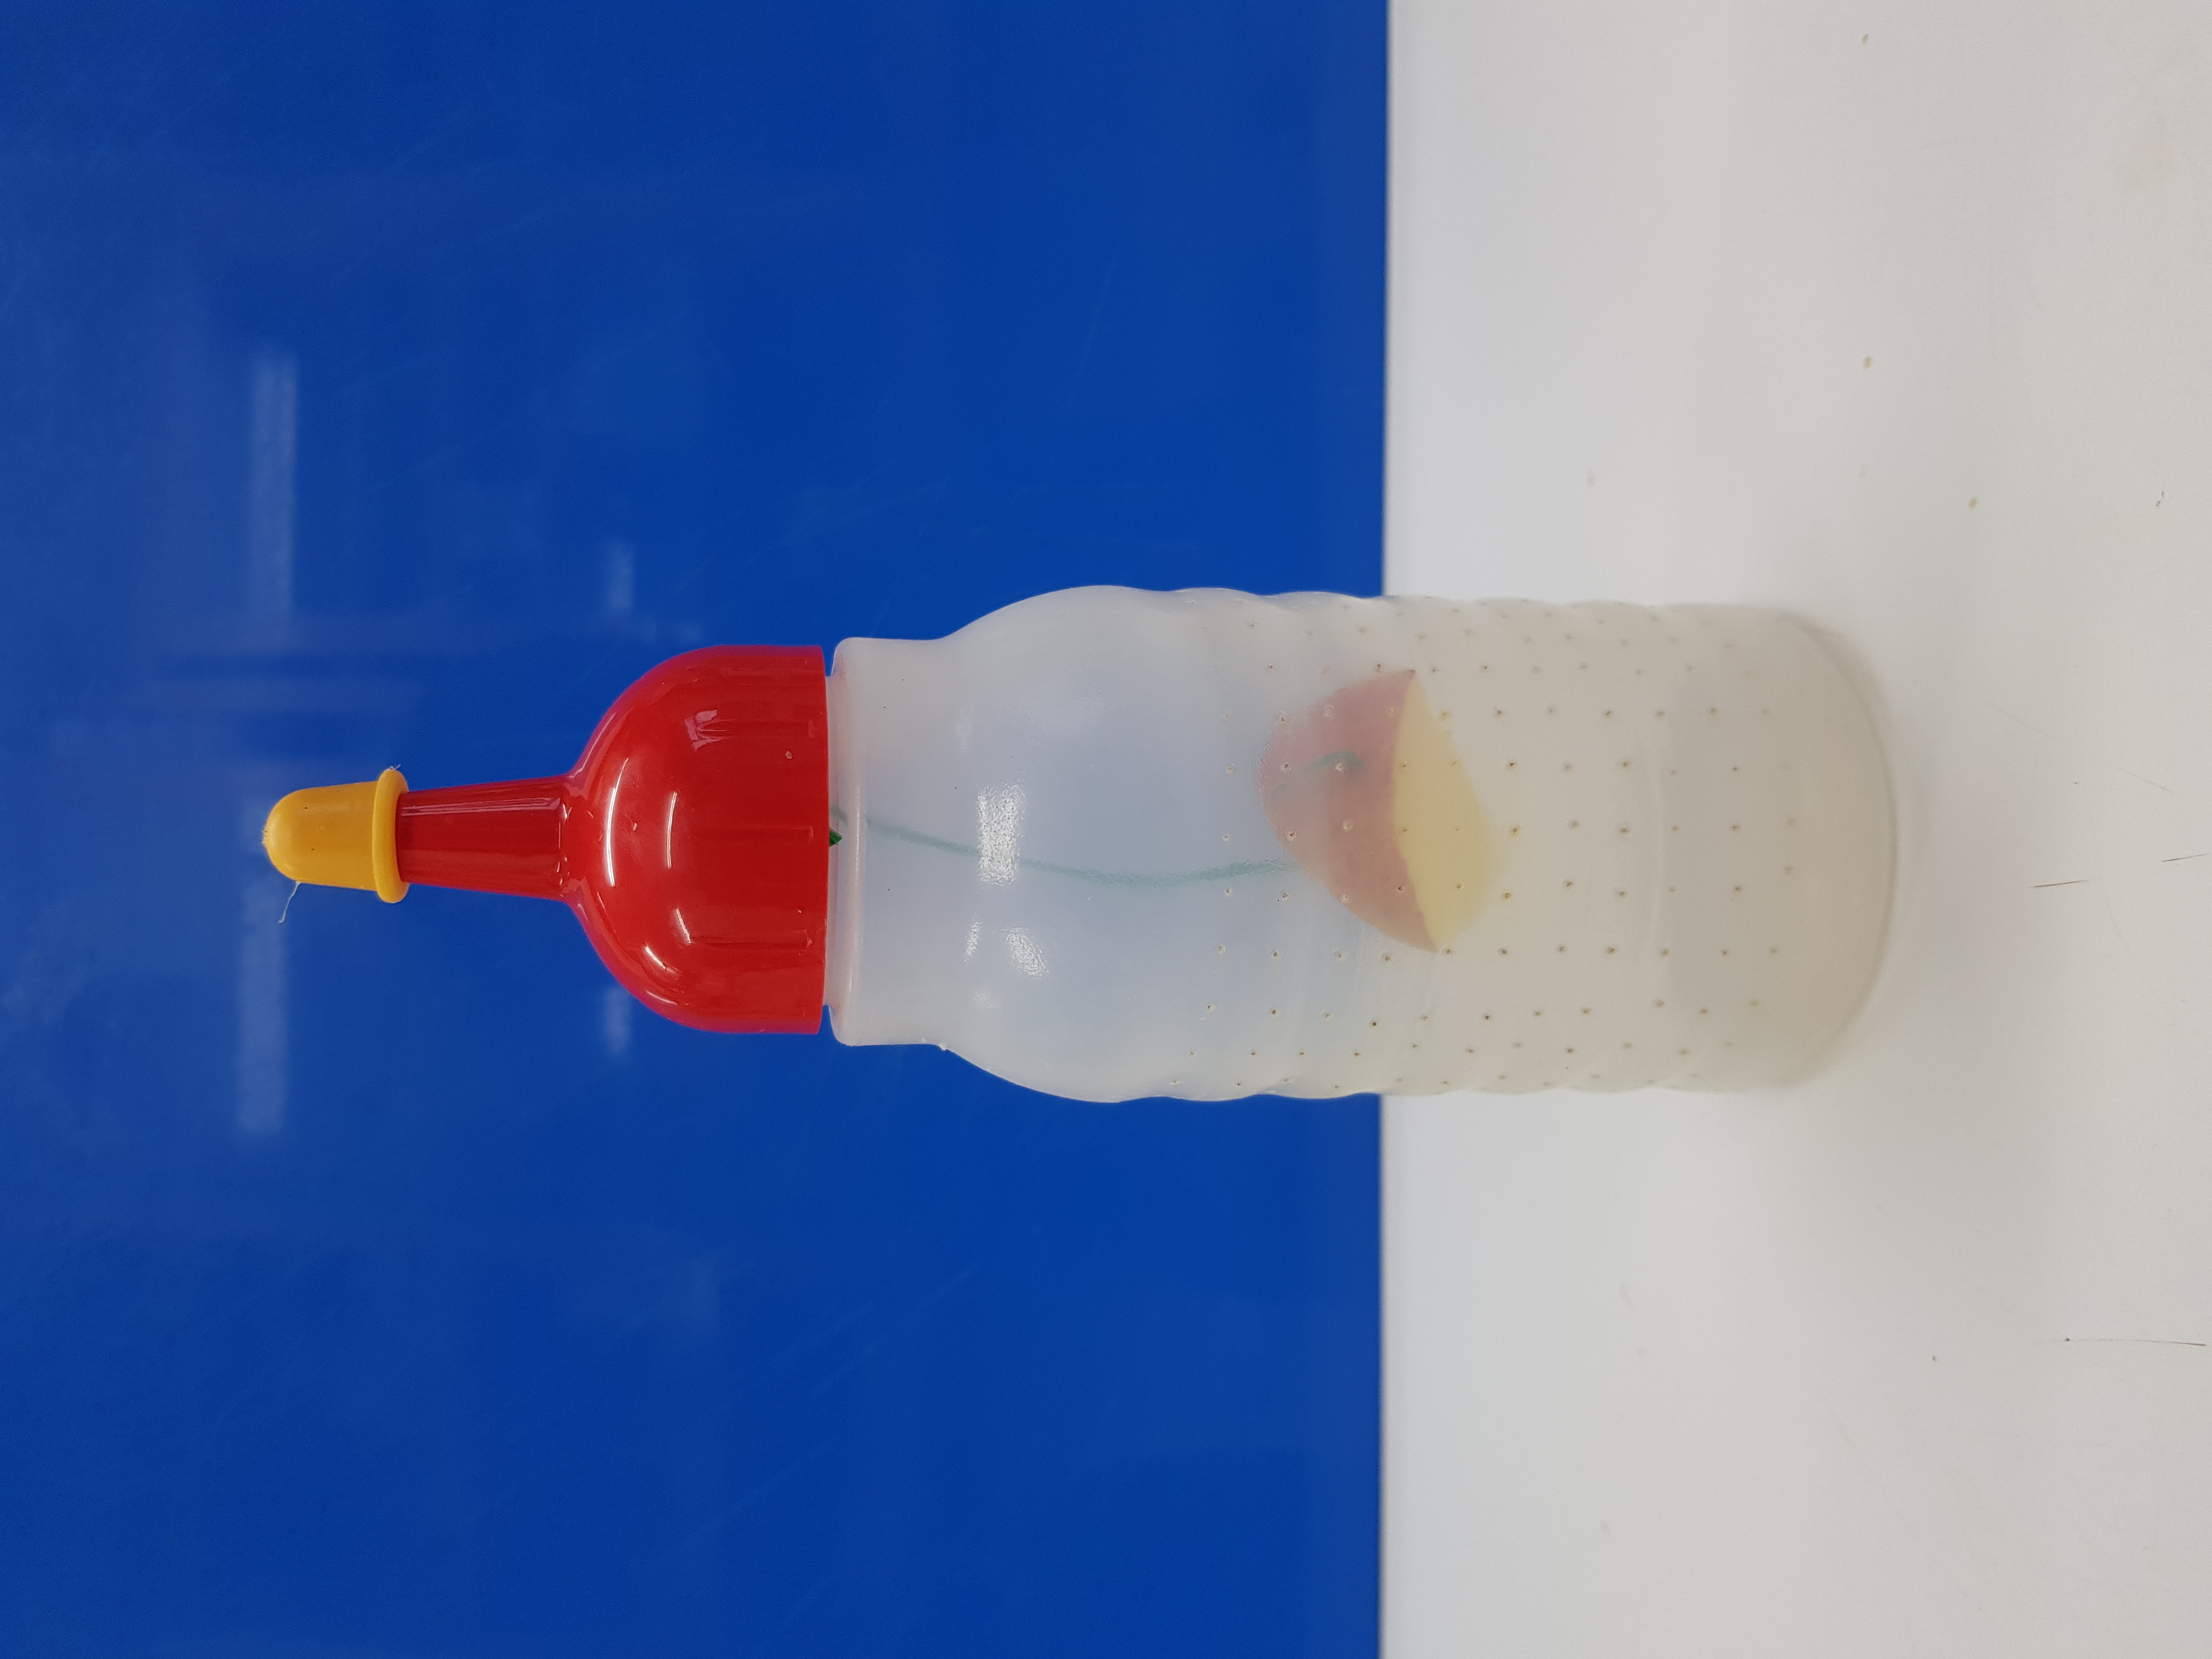
\includegraphics[width=0.8\linewidth,angle=270]{Supplementary_files/figure-latex/Egging_device} 

}

\caption{Picture of the egging device.}\label{fig:FigS1 Heat units}
\end{figure}

\newpage

\begin{figure}

{\centering \includegraphics{Supplementary_files/figure-latex/FigS2-1} 

}

\caption{Results pilot experiment on heat knockdown time. Data are presented as knockdown time in minutes on two different exposure temperature for S06 flies. Significance differences of means between temperatures are reported with Wilcox test P-value.}\label{fig:FigS2}
\end{figure}\newpage

\blandscape

\begin{figure}

{\centering \includegraphics{Supplementary_files/figure-latex/Units_for_chill_coma_recovery_assay} 

}

\caption{Units for cold recovery treatment}\label{fig:FigS3 Cold units}
\end{figure}

\elandscape

\newpage

\blandscape

\begin{figure}

{\centering \includegraphics[width=0.9\linewidth]{Supplementary_files/figure-latex/Weather variables correlation for selection-1} 

}

\caption{\textbf{Correlation among 11 climatic variables}. Correlation values are presented together with asterisk indicating signficance values for each correlation. Variables names are indicative of the following weather variables: \textbf{mean.max}= Annual max temperature; \textbf{mean.min} = Annual mim temperature; \textbf{mean.rain} = Annual rainfall; \textbf{mean.solar}= Annual solar exposure; annual.temp = Annual temperature; max.high.temp = Maximum temperature of the warmest month; low.high.temp = Mimimum temperature of the warmest month; low.min.temp = Minimum temperature of the coldest month; \textbf{high.min.temp} = Minimum temperature of the coldest month; \textbf{min.dry.month}= Precipitation of the driest month; \textbf{max.wet.month} = Precipitation of the wettest month.}\label{fig:Weather variables correlation for selection}
\end{figure}

\elandscape

\begin{figure}

{\centering \includegraphics{Supplementary_files/figure-latex/Diagnostic plots heat tolerance wild flies-1} 

}

\caption{Diagnostic plots Gamma-GLM heat tolerance in wild populations of the Queensland fruit fly}\label{fig:Diagnostic plots heat tolerance wild flies}
\end{figure}

\begin{figure}

{\centering \includegraphics{Supplementary_files/figure-latex/Diagnostic plots heat tolerance in domesticated flies-1} 

}

\caption{Diagnostic plots Gamma-GLM heat tolerance in domesticated populations of the Queensland fruit fly}\label{fig:Diagnostic plots heat tolerance in domesticated flies}
\end{figure}

\begin{figure}

{\centering \includegraphics{Supplementary_files/figure-latex/Diagnostic plots heat tolerance during domestication-1} 

}

\caption{Diagnostic plots Gamma-GLM heat tolerance change during domestication}\label{fig:Diagnostic plots heat tolerance during domestication}
\end{figure}

\begin{figure}

{\centering \includegraphics{Supplementary_files/figure-latex/Diagnostic plots cold tolerance wild flies-1} 

}

\caption{Diagnostic plots Gamma-GLM cold tolerance in wild populations of the Queensland fruit fly}\label{fig:Diagnostic plots cold tolerance wild flies}
\end{figure}

\begin{figure}

{\centering \includegraphics{Supplementary_files/figure-latex/Diagnostic plots cold tolerance in domesticated flies-1} 

}

\caption{Diagnostic plots Gamma-GLM heat tolerance in domesticated populations of the Queensland fruit fly}\label{fig:Diagnostic plots cold tolerance in domesticated flies}
\end{figure}

\begin{figure}

{\centering \includegraphics{Supplementary_files/figure-latex/Diagnostic plots cold tolerance during domestication-1} 

}

\caption{Diagnostic plots Gamma-GLM cold tolerance change during domestication}\label{fig:Diagnostic plots cold tolerance during domestication}
\end{figure}

\begin{figure}

{\centering \includegraphics{Supplementary_files/figure-latex/Diagnostic plots desiccation wild populations-1} 

}

\caption{Diagnostic plots Gamma-GLM desiccation tolerance in wild Qfly populations}\label{fig:Diagnostic plots desiccation wild populations}
\end{figure}

\begin{figure}

{\centering \includegraphics{Supplementary_files/figure-latex/Diagnostic plots desiccation tolerance in domesticated flies-1} 

}

\caption{Diagnostic plots Gamma-GLM desiccation tolerance in domesticated populations of the Queensland fruit fly}\label{fig:Diagnostic plots desiccation tolerance in domesticated flies}
\end{figure}

\begin{figure}

{\centering \includegraphics{Supplementary_files/figure-latex/Diagnostic plots desiccation change during domestication-1} 

}

\caption{Diagnostic plots Gamma-GLM desiccation tolerance change during domestication}\label{fig:Diagnostic plots desiccation change during domestication}
\end{figure}

\begin{figure}

{\centering \includegraphics{Supplementary_files/figure-latex/Diagnostic plots starvation wild populations-1} 

}

\caption{Diagnostic plots Gamma-GLM starvation tolerance in wild Qfly populations}\label{fig:Diagnostic plots starvation wild populations}
\end{figure}

\begin{figure}

{\centering \includegraphics{Supplementary_files/figure-latex/Diagnostic plots starvation tolerance in domesticated flies-1} 

}

\caption{Diagnostic plots Gamma-GLM starvation tolerance in domesticated populations of the Queensland fruit fly}\label{fig:Diagnostic plots starvation tolerance in domesticated flies}
\end{figure}

\begin{figure}

{\centering \includegraphics{Supplementary_files/figure-latex/Diagnostic plots starvation change during domestication-1} 

}

\caption{Diagnostic plots Gamma-GLM starvation tolerance change during domestication}\label{fig:Diagnostic plots starvation change during domestication}
\end{figure}

\blandscape
\elandscape
\#\#\# R session information:

\begin{verbatim}
## R version 3.4.4 (2018-03-15)
## Platform: x86_64-pc-linux-gnu (64-bit)
## Running under: Ubuntu 16.04.6 LTS
## 
## Matrix products: default
## BLAS: /usr/lib/openblas-base/libblas.so.3
## LAPACK: /usr/lib/libopenblasp-r0.2.18.so
## 
## locale:
##  [1] LC_CTYPE=en_AU.UTF-8       LC_NUMERIC=C              
##  [3] LC_TIME=en_AU.UTF-8        LC_COLLATE=en_AU.UTF-8    
##  [5] LC_MONETARY=en_AU.UTF-8    LC_MESSAGES=en_AU.UTF-8   
##  [7] LC_PAPER=en_AU.UTF-8       LC_NAME=C                 
##  [9] LC_ADDRESS=C               LC_TELEPHONE=C            
## [11] LC_MEASUREMENT=en_AU.UTF-8 LC_IDENTIFICATION=C       
## 
## attached base packages:
## [1] grid      stats     graphics  grDevices utils     datasets  methods  
## [8] base     
## 
## other attached packages:
##  [1] PerformanceAnalytics_1.5.2 xts_0.11-2                
##  [3] zoo_1.8-5                  pander_0.6.3              
##  [5] emmeans_1.3.3              boot_1.3-20               
##  [7] nortest_1.0-4              jtrans_0.2.1              
##  [9] Hmisc_4.2-0                Formula_1.2-3             
## [11] survival_2.42-6            lattice_0.20-35           
## [13] xtable_1.8-3               psych_1.8.12              
## [15] egg_0.4.2                  gridExtra_2.3             
## [17] sp_1.3-1                   purrr_0.3.2               
## [19] cowplot_0.9.4              ggpubr_0.2                
## [21] magrittr_1.5               ggridges_0.5.1            
## [23] ggplot2_3.1.0              readr_1.3.1               
## [25] dplyr_0.8.0.1              wesanderson_0.3.6         
## 
## loaded via a namespace (and not attached):
##  [1] httr_1.4.0          viridisLite_0.3.0   splines_3.4.4      
##  [4] assertthat_0.2.1    latticeExtra_0.6-28 yaml_2.2.0         
##  [7] pillar_1.3.1        backports_1.1.3     quadprog_1.5-5     
## [10] glue_1.3.1          digest_0.6.18       RColorBrewer_1.1-2 
## [13] ggsignif_0.5.0      checkmate_1.9.1     rvest_0.3.2        
## [16] colorspace_1.4-1    htmltools_0.3.6     Matrix_1.2-14      
## [19] plyr_1.8.4          pkgconfig_2.0.2     mvtnorm_1.0-8      
## [22] scales_1.0.0        webshot_0.5.1       htmlTable_1.13.1   
## [25] tibble_2.1.1        withr_2.1.2         nnet_7.3-12        
## [28] lazyeval_0.2.2      mnormt_1.5-5        crayon_1.3.4       
## [31] estimability_1.3    evaluate_0.13       nlme_3.1-137       
## [34] xml2_1.2.0          foreign_0.8-70      tools_3.4.4        
## [37] data.table_1.12.0   hms_0.4.2           stringr_1.4.0      
## [40] munsell_0.5.0       cluster_2.0.7-1     packrat_0.5.0      
## [43] kableExtra_1.1.0    compiler_3.4.4      rlang_0.3.2        
## [46] rstudioapi_0.10     htmlwidgets_1.3     base64enc_0.1-3    
## [49] labeling_0.3        rmarkdown_1.12      gtable_0.3.0       
## [52] R6_2.4.0            knitr_1.22          stringi_1.4.3      
## [55] parallel_3.4.4      Rcpp_1.0.1          rpart_4.1-13       
## [58] acepack_1.4.1       tidyselect_0.2.5    xfun_0.5           
## [61] coda_0.19-2
\end{verbatim}


\end{document}
